\subsection{Transconductance Amplifier Function}

We can now start to analyze the dynamics when both the current mirror and the diff pair are connected to form a transconductance amplifier.

\subsubsection{Let's assume everything is in Saturation}

Let's first start with, as always, some assumptions and consequent observations. 
\begin{itemize}
    \item $M_1$ works in saturation: $I_1 = I_0 e^{\frac{\kappa V_1 - V_S}{U_T}}$
    \item $M_2$ works in saturation: $I_2 = I_0 e^{\frac{\kappa V_2 - V_S}{U_T}}$
    \item $M_3$ works in saturation: $I_b = I_0 e^{\frac{\kappa V_b}{U_T}}$
    \item $M_4$ and $M_5$ are also in saturation. We can therefore apply the P-Type current mirror equation reached previously. 
\end{itemize}

Now let's see what we can reach with this. We noted previously that our current mirror had a unity gain, this means that $I_1$ flows through $M_5$ (since it is mirroring the current of $M4$). Using Kirchoff's current law, we can now establish that: $I_{out} = I_1 - I_2$. If we take the expression derived in the assumptions for $I_1$ and $I_2$, we reach with some tedious algebra: 

\begin{equation}
    I_{out} = I_1 - I_2 = I_b\frac{e^{\frac{\kappa V_1}{U_T}} - e^{\frac{\kappa V_2}{U_T}}}{e^{\frac{\kappa V_1}{U_T}} + e^{\frac{\kappa V_2}{U_T}}} = I_b \mathrm{tanh}(\frac{\kappa (V_1 - V_2)}{2U_T}) 
\end{equation}

This yields the following dynamic: 

\begin{figure}[H]
    \centering
    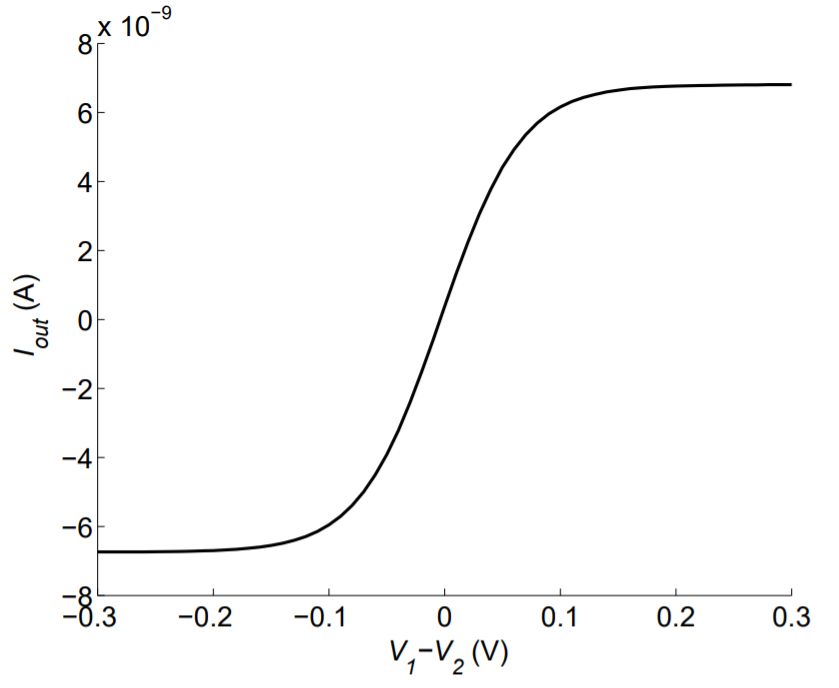
\includegraphics[width=0.5\linewidth]{../../Figures/Saturation_Transconductance_Amp.PNG}
    \caption{The Transconductance Amplifier ouptput current as a function of the difference between $V_1$ and $V_2$. This is assuming that all transistors, especially $M_3$ are in saturation. Adapted from Lecture Notes.}
    \label{fig:_saturated_transconductance_amplifier}
\end{figure}

Importantly, we note that for small differential voltages ($|V_1 - V_2|\ < 200 \textrm{mv}$), the tanh relationship is approximately linear and our equation can be reduced to: 

\begin{equation}
    I_{out} \approx g_m(V_1 - V_2) \ \mathrm{with} \ g_m = \frac{I_b \kappa}{2 U_T}
\end{equation}

The term $g_m$ is the \textbf{transconductance} of the amplifier. It quantifies how much the potential difference will influence the output current. It has the dimensions of a conductance (1/Ohms). To increase $g_m$, you can only increase $I_b$. Usually, a high transconductance is more desirable, as it leads to a higher out current for the same current. The issue is that to increase $I_b$, you need a higher $V_b$, which means consuming more energy. As Shih-Chii says: there is no free lunch!
Because the output current is measured at a terminal which is different from the pair across which the input voltage difference is applied, we can also define another term (which we've defined before!): the \textbf{output conductance $g_d$}. Instead of measuring the change in current as a function of \textit{input} voltage as with $g_m$, we measure the change in current as a function of the change in \textit{output} voltage. We reach the familiar expression: 

\begin{equation}
    g_d = - \frac{\partial I_{out}}{\partial V_{out}} \approx \frac{I_b}{V_E}
\end{equation}

where $V_E$ is the Early Voltage of $M_2$ and $M_5$, assumed equal. 

\subsubsection{Let's stop assuming that everything is in Saturation}

Now, let's consider the case where we cannot assume that $M_3$ operates in saturation (does not mean it is not in saturation, just that we cannot assume it). This yields a different behaviour. We assume that the rest is still in saturation. We therefore have to write the full equation for current $I_b$.

\begin{equation}
    I_b = I_0 e^{\frac{\kappa V_b}{U_T}}(1 - e^{\frac{-V_s}{U_T}})
\end{equation}

From the differential pair, we know that $I_b$ = $I_1$ + $I_2$. Assuming that $M_1$ and $M_2$ are in saturation, we reach: 

\begin{equation}
    I_b = I_0 e^{\frac{\kappa V_b}{U_T}}(1 - e^{\frac{-V_s}{U_T}}) = I_0e^{\frac{\kappa V_1 - V_s}{U_T}} + I_0e^{\frac{\kappa V_2 - V_s}{U_T}}
\end{equation}

Solving for $e^{-V_s/U_T}$, we reach with some, as always, tedious algebra: 

\begin{equation}
    e^{-V_s/U_T} = \frac{e^{\kappa V_b/U_T}}{e^{\kappa V_b/U_T} + e^{\kappa V_1/U_T} + e^{\kappa V_2/U_T}}
\end{equation}

So we considered the case where we could not be certain of $M_3$ operating in saturation. We derived the subsequent equation, and now we want to find what are the conditions and implications of $M_3$ actually being in saturation. Confusing, I know. But just think of it as a more rigorous way to work with this circuit: we want $M_3$ to be in saturation but we can't assume it is, so let's figure out how to make it work the way we want. So: if we want $M_3$ to operate in saturation, we need the $V_{ds}$ of $M_3$ to be above $4 U_T$, which means that $V_s > 4U_T$  and subsequently that $e^{-V_s/U_T} << 1$. Now let's do some maths: 

\begin{equation}
    e^{-V_s/U_T} = \frac{e^{\kappa V_b/U_T}}{e^{\kappa V_b/U_T} + e^{\kappa V_1/U_T} + e^{\kappa V_2/U_T}} << 1
\end{equation}
\begin{equation}
    e^{\kappa V_b/U_T} << e^{\kappa V_b/U_T} + e^{\kappa V_1/U_T} + e^{\kappa V_2/U_T}
\end{equation}
If we divide both sides by $e^{\kappa V_b/U_T}$, we reach: 
\begin{equation}
    1 + \frac{e^{\kappa V_1/U_T} + e^{\kappa V_2/U_T}}{e^{\kappa V_b/U_T}} >> 1
\end{equation}
\begin{equation}
    \frac{e^{\kappa V_1/U_T} + e^{\kappa V_2/U_T}}{e^{\kappa V_b/U_T}} >> 1
\end{equation}

Remember that: 

\begin{equation}
    e^{-V_s/U_T} = \frac{e^{\kappa V_b/U_T}}{e^{\kappa V_b/U_T} + e^{\kappa V_1/U_T} + e^{\kappa V_2/U_T}}
\end{equation}

Well from, that, we can derive $V_s$: 

\begin{equation}
    V_s = -\kappa V_b + U_T \ \mathrm{ln}(e^{\kappa V_b/U_T} + e^{\kappa V_1/U_T} + e^{\kappa V_2/U_T})
\end{equation}

Which, thanks to equation 49, yields: 

\begin{equation}
    V_s = -\kappa V_b + U_T \ \mathrm{ln}(e^{\kappa V_1/U_T} + e^{\kappa V_2/U_T})
\end{equation}

Now, taking the assumption that $|V_1 - V_2| > 4 U_T$, we can finally turn into something useful:

\begin{equation}
    V_s \approx \kappa (\textrm{max}(V1,V2) - V_b)
\end{equation}

Wait what? Where did the max come from? Yeah I asked myself the same question. It's no difficult to see: because the difference between $|V_1 - V_2| > 4 U_T $, the expression inside the logarithm will converge to whichever of $V_1$ or $V_2$ is the biggest, hence the max function. Then it's just some factorizing to do. Well anyways, now we managed to derive what condition we need to satisfy to ensure that $M_3$ will be in saturation as it will have $V_S > 4 U_T$:
\begin{equation}
    \textrm{max}(V1,V2) > V_b + \frac{4U_T}{\kappa}
\end{equation}
Yes, all of this, just to know what kind of voltage we have to apply to $V1$, $V2$ and $V_B$ so that our transistor $M_3$ is in saturation. Now we can use the equation we derive in the previous section, without feeling bad about the fact we're just doing something unrealistic as we have too many assumptions. You see, assumptions aren't so bad in the end?  And yes, I know, that was all very tedious, and probably unnecessary to derive here as we clearly won't have to do that for the exam. But don't get mad, I'm just trying to give you all the good info, and it's 2 in the morning so I am not thinking straight. 

\paragraph{But what about the other Transistors?}

Before we move on, let's have a last look at the assumptions. So we just managed to derive the specific conditions to satisfy to ensure that $M_3$ operates in saturation. We, unfortunately, have to consider the saturation conditions for the other transistors as well. For practical purposes, $M_1$ and $M_4$ will always be in saturation because $M_4$ is \textit{diode-connected} and the drain of $M_1$ is thus at a high voltage (THIS IS WORD TO WORD WHAT IS WRITTEN IN THE TEXTBOOK, BUT SHOULDN'T IT BE LOW VOLTAGE?). Now we need to look at $M_2$ and $M_5$. So for these we're gonna have to work on it a bit. 
\begin{itemize}
    \item To keep $M_5$ in saturation, we need $V_{dd}$ - $V_{out} > 4 U_T$
    \item To keep $M_2$ in saturation, we need $V_{out}$ - $V_{s} > 4 U_T \equiv V_{out} > 4 U_T +  V_S$. We've just found $V_S$ before, so let's use that, and we get
    \begin{equation}
        V_{out} > \kappa (\mathrm{max}(V_1, V_2) - V_b) + 4 U_T
    \end{equation}
    Huh... That's annoying. Our $V_{out}$ also need to satisfy some condition which depends on $V_1$, $V_2$ and $V_b$. This is called the min problem, because we manage to get in saturation only if the \textit{minimum} $V_{out}$ is greater than the condition above. And well, before we kinda also reached a min problem where we had saturation only if $|V_1 - V_2|$ was higher than $V_b + 4U_T/ \kappa$. So you see that to get this circuit operated properly, you need to satisfy a lot of different things, which in practice are absolutely not trivial to satisfy. 
    \item So how does this circuit work in practice? To be honest I am not sure myself and wouldn't mind having your input on it :). 
\end{itemize}


\subsubsection{Transconductance Amplifier as a Voltage Amplifier}\label{sec:transamp_voltage}

This will be a brief comment on the subject. There is more to know than what we'll discuss, but we are not required to know the details. The transconductance amplifier can be used as a differential input voltage amplifier, where essentially: $V_{out} = A(V_1 - V_2)$. A being the gain of the circuit, relating the change in output compared to the change in input. Here is the transfer function, which uses some of our previously derived knowledge on transconductance and output conductance: 

\begin{equation}
    A = \frac{\partial{V_{out}}}{\partial{(V_1 - V_2)}} = \frac{\partial {V_{out}}}{\partial{I_{out}}} \frac{\partial {I_{out}}}{\partial{(V_1 - V_2)}} = \frac{g_m}{g_d} \approx \frac{\kappa V_E}{2U_T}
\end{equation}

Here are key take aways from how this amplifier works: 

\begin{itemize}
    \item The oper-circuit voltage gain A increases with Early Voltage and therefore with the length of the output transistors.
    \item Typical subthreshold values of A are between 100 and 1000.
    \item Because of the large voltage gain and transistor mismatch effects, the amplifier is usually used in a negative-feedback configuration. WHAT DOES THIS MEAN?
    \item In open-voltage mode, it is used mainly as a comparator: $V_{out}$ is "high" only when $V_1 > V_2$, and vice versa. 
\end{itemize}


Ok that was a lot for just one circuit. Let's summarize the key take aways: 

\begin{itemize}
    \item $M_3$ cannot be assumed to be in Saturation, so we used the full subtrehshold equation to find under what conditions $M_3$ could indeed be in saturation. We found that we needed to tune $V_1$, $V_2$ and $V_b$ to ensure that $\textrm{max}(V1,V2) > V_b + \frac{4U_T}{\kappa}$ to be in saturation. If we do tune our voltages according to this equation, we are in saturation, and the I-V relationship derived in the previous section applies. 
    \item 
\end{itemize}

THIS SENTENCE NEEDS TO BE SOMEWHERE:

Since Vout increases with increasing V1 and decreases with increasing V2,
the gate of M1 is called the non-inverting input terminal and the gate of
M2 the inverting input terminal of the amplifier.